\chapter{Appendix}
\label{ap: Penalty}

Extending the idea of \eqref{eq:penalty_function}, one can devise a more highly nonlinear versions of the penalty functional. For example, from

\begin{equation}
\frac{\partial^2 U_2(J;\beta)}{\partial J^2} = \beta(J-1)^4 + 1,
\end{equation}

we can derive 
\begin{align}
\frac{\partial U_2(J;\beta)}{\partial J} &= \frac{1}{5} (J-1) \left[ \beta(J-1)^4 + 5 \right], and \\
U_2(J;\beta) &= \frac{1}{30} (J-1)^2 \left[ \beta (J-1)^4 + 15 \right].
\end{align}

In this sense, we can derive a penalty function of arbitrary order, based on the second derivative. To satisfy condition \textbf{e} from Section~\ref{ch:Volume Penalty}, the order of the second derivative must be an even number, so for a natural number $n$ one can define a second derivative as

\begin{equation}
\frac{\partial^2 U_n(J;\beta)}{\partial J^2} = \beta(J-1)^{2n} + 1,
\end{equation}

then build the penalty function $U_n(J; \beta)$ that satisfies all the five conditions from the second derivative as follows,

\begin{equation}
U_n(J;\beta) = \frac{1}{(2n+1)(2n+2)} (J-1)^2 \left[ \beta (J-1)^{2n} + \frac{(2n+1)(2n+2)}{2} \right].
\end{equation}

We plot the runtimes and average Ipopt iterations for the first few $n$ of these penalties, for the cube twist simulation in Figure~\ref{fig:penalty_comparison}, with $\beta = 1$.
Notice how the runtime and number of iterations increase linearly depending on $n$. 
From this simple experiment, we can conclude that although the added nonlinearity of the gradient is beneficial for resolving tet inversions, additional nonlinearity of the energy is actually harmful for the performance. Therefore, we argue that our choice of the penalty functional in \eqref{eq:penalty_function} is indeed optimal for our purposes.

\begin{figure}[t] 
	\centering
	\begin{subfigure}{.49\linewidth}
		\centering 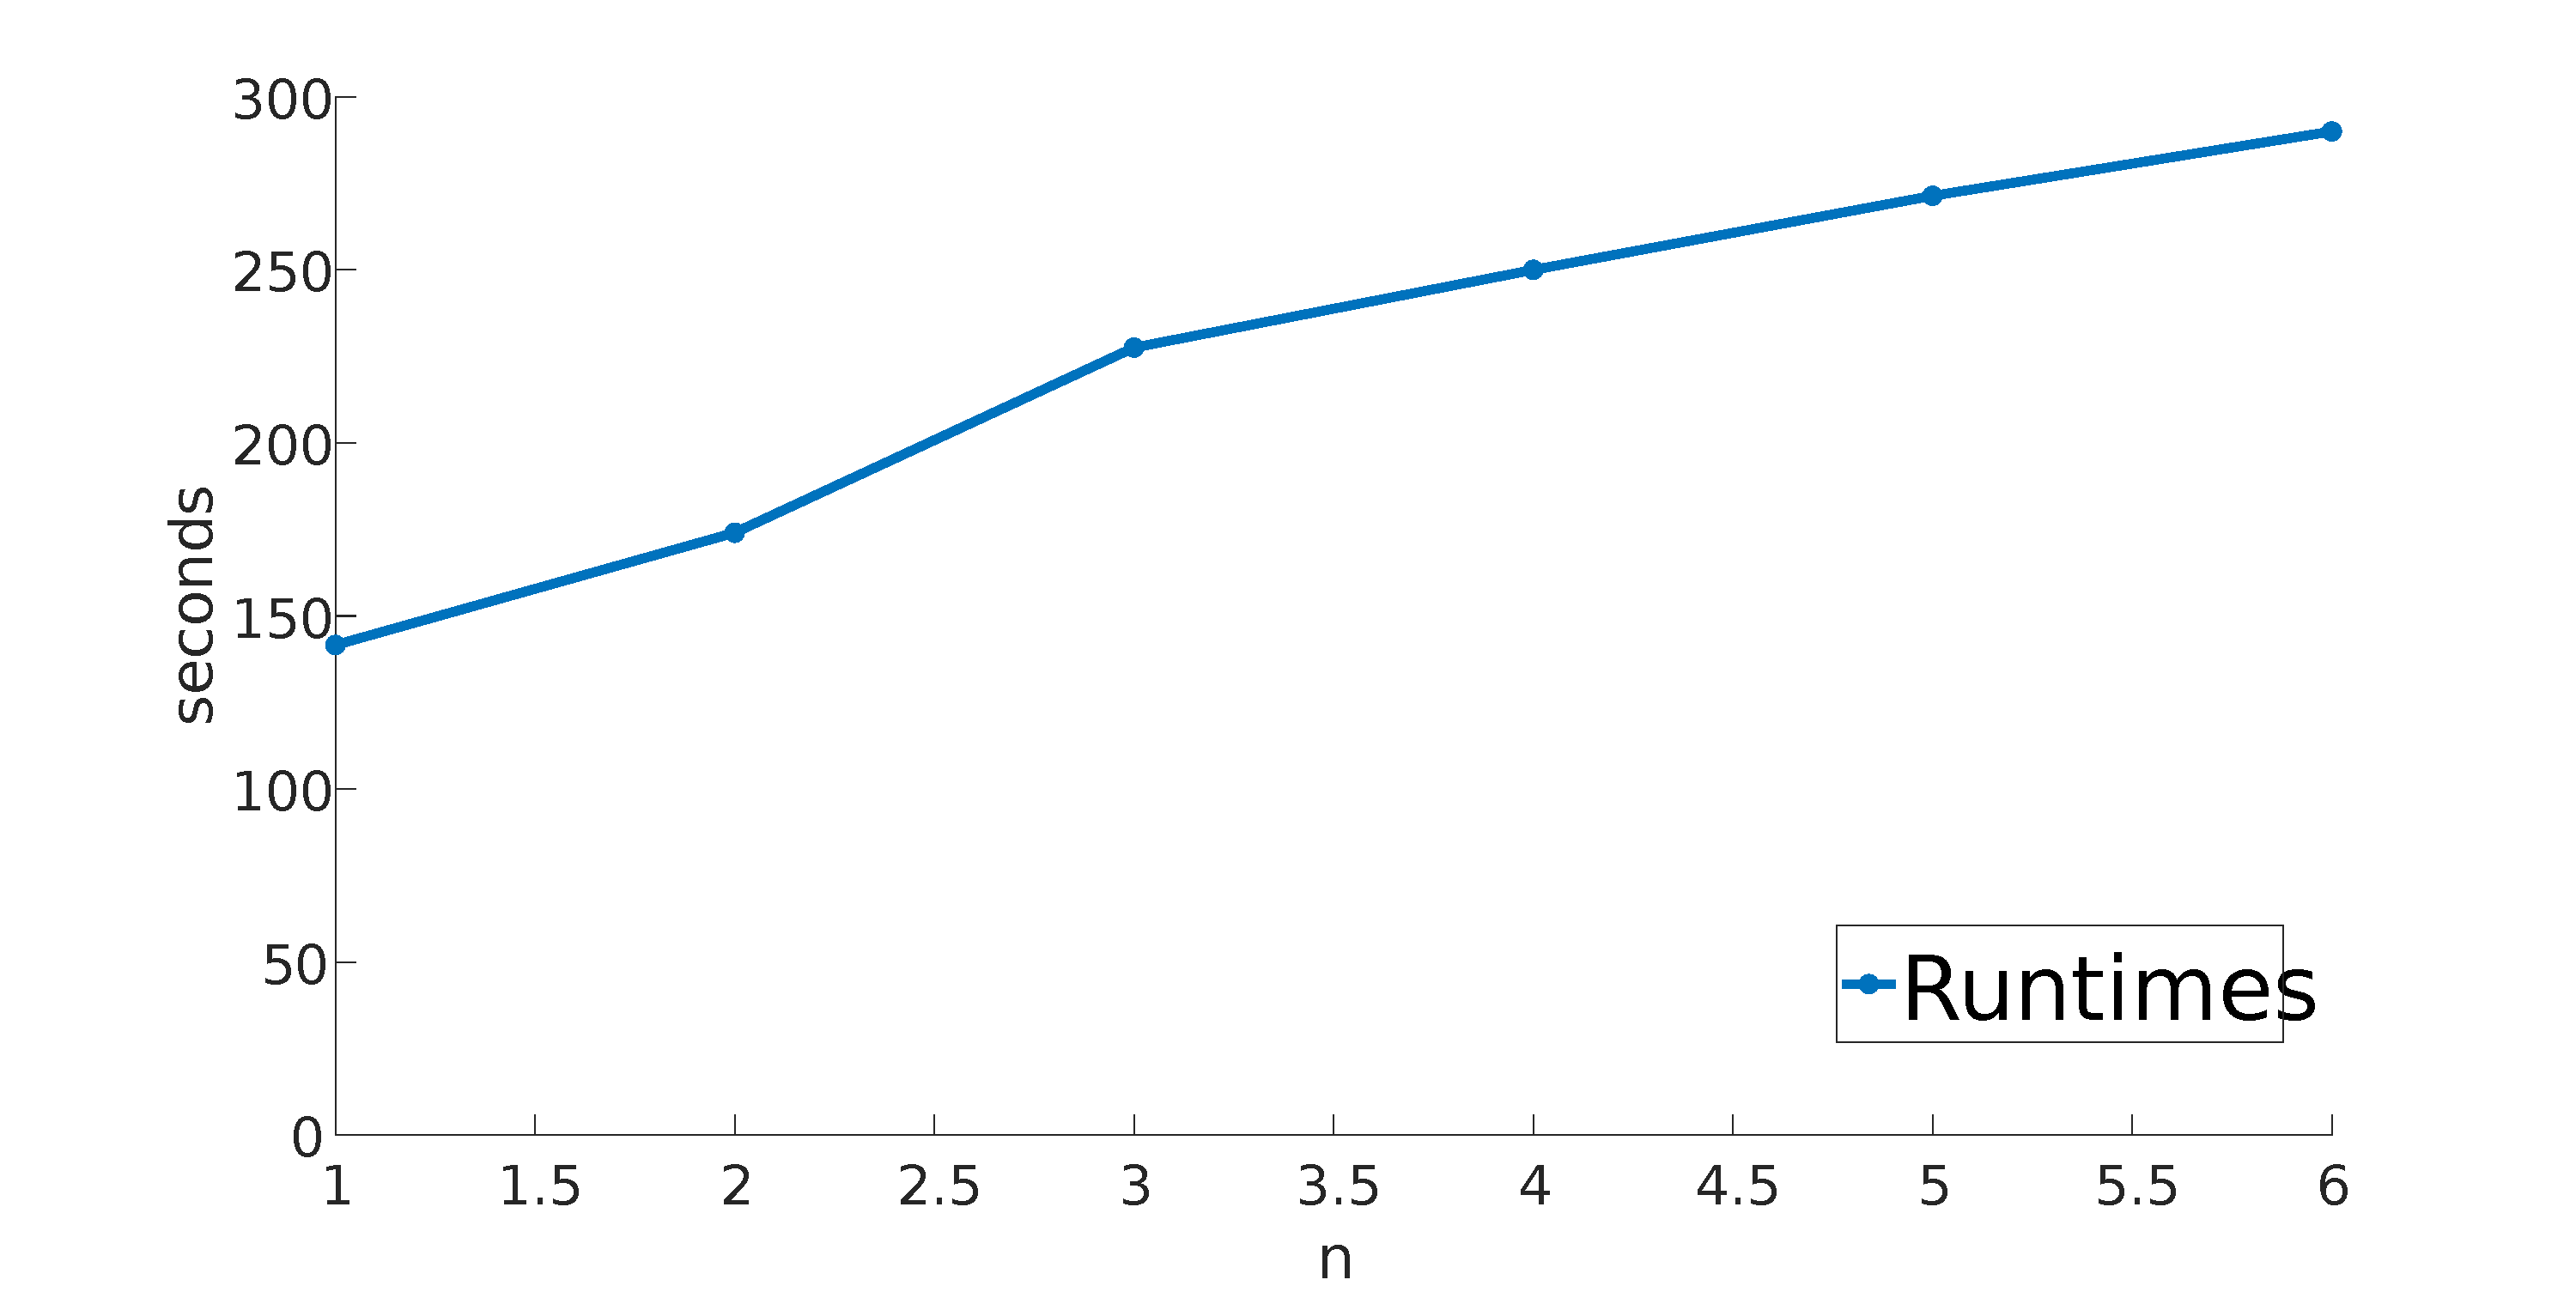
\includegraphics[width=2.5in]{images/penalty_runtimes.pdf}
		\caption*{(a)}
		\label{sfig:pen_runtimes}
	\end{subfigure}%
	\begin{subfigure}{.49\linewidth}
		\centering 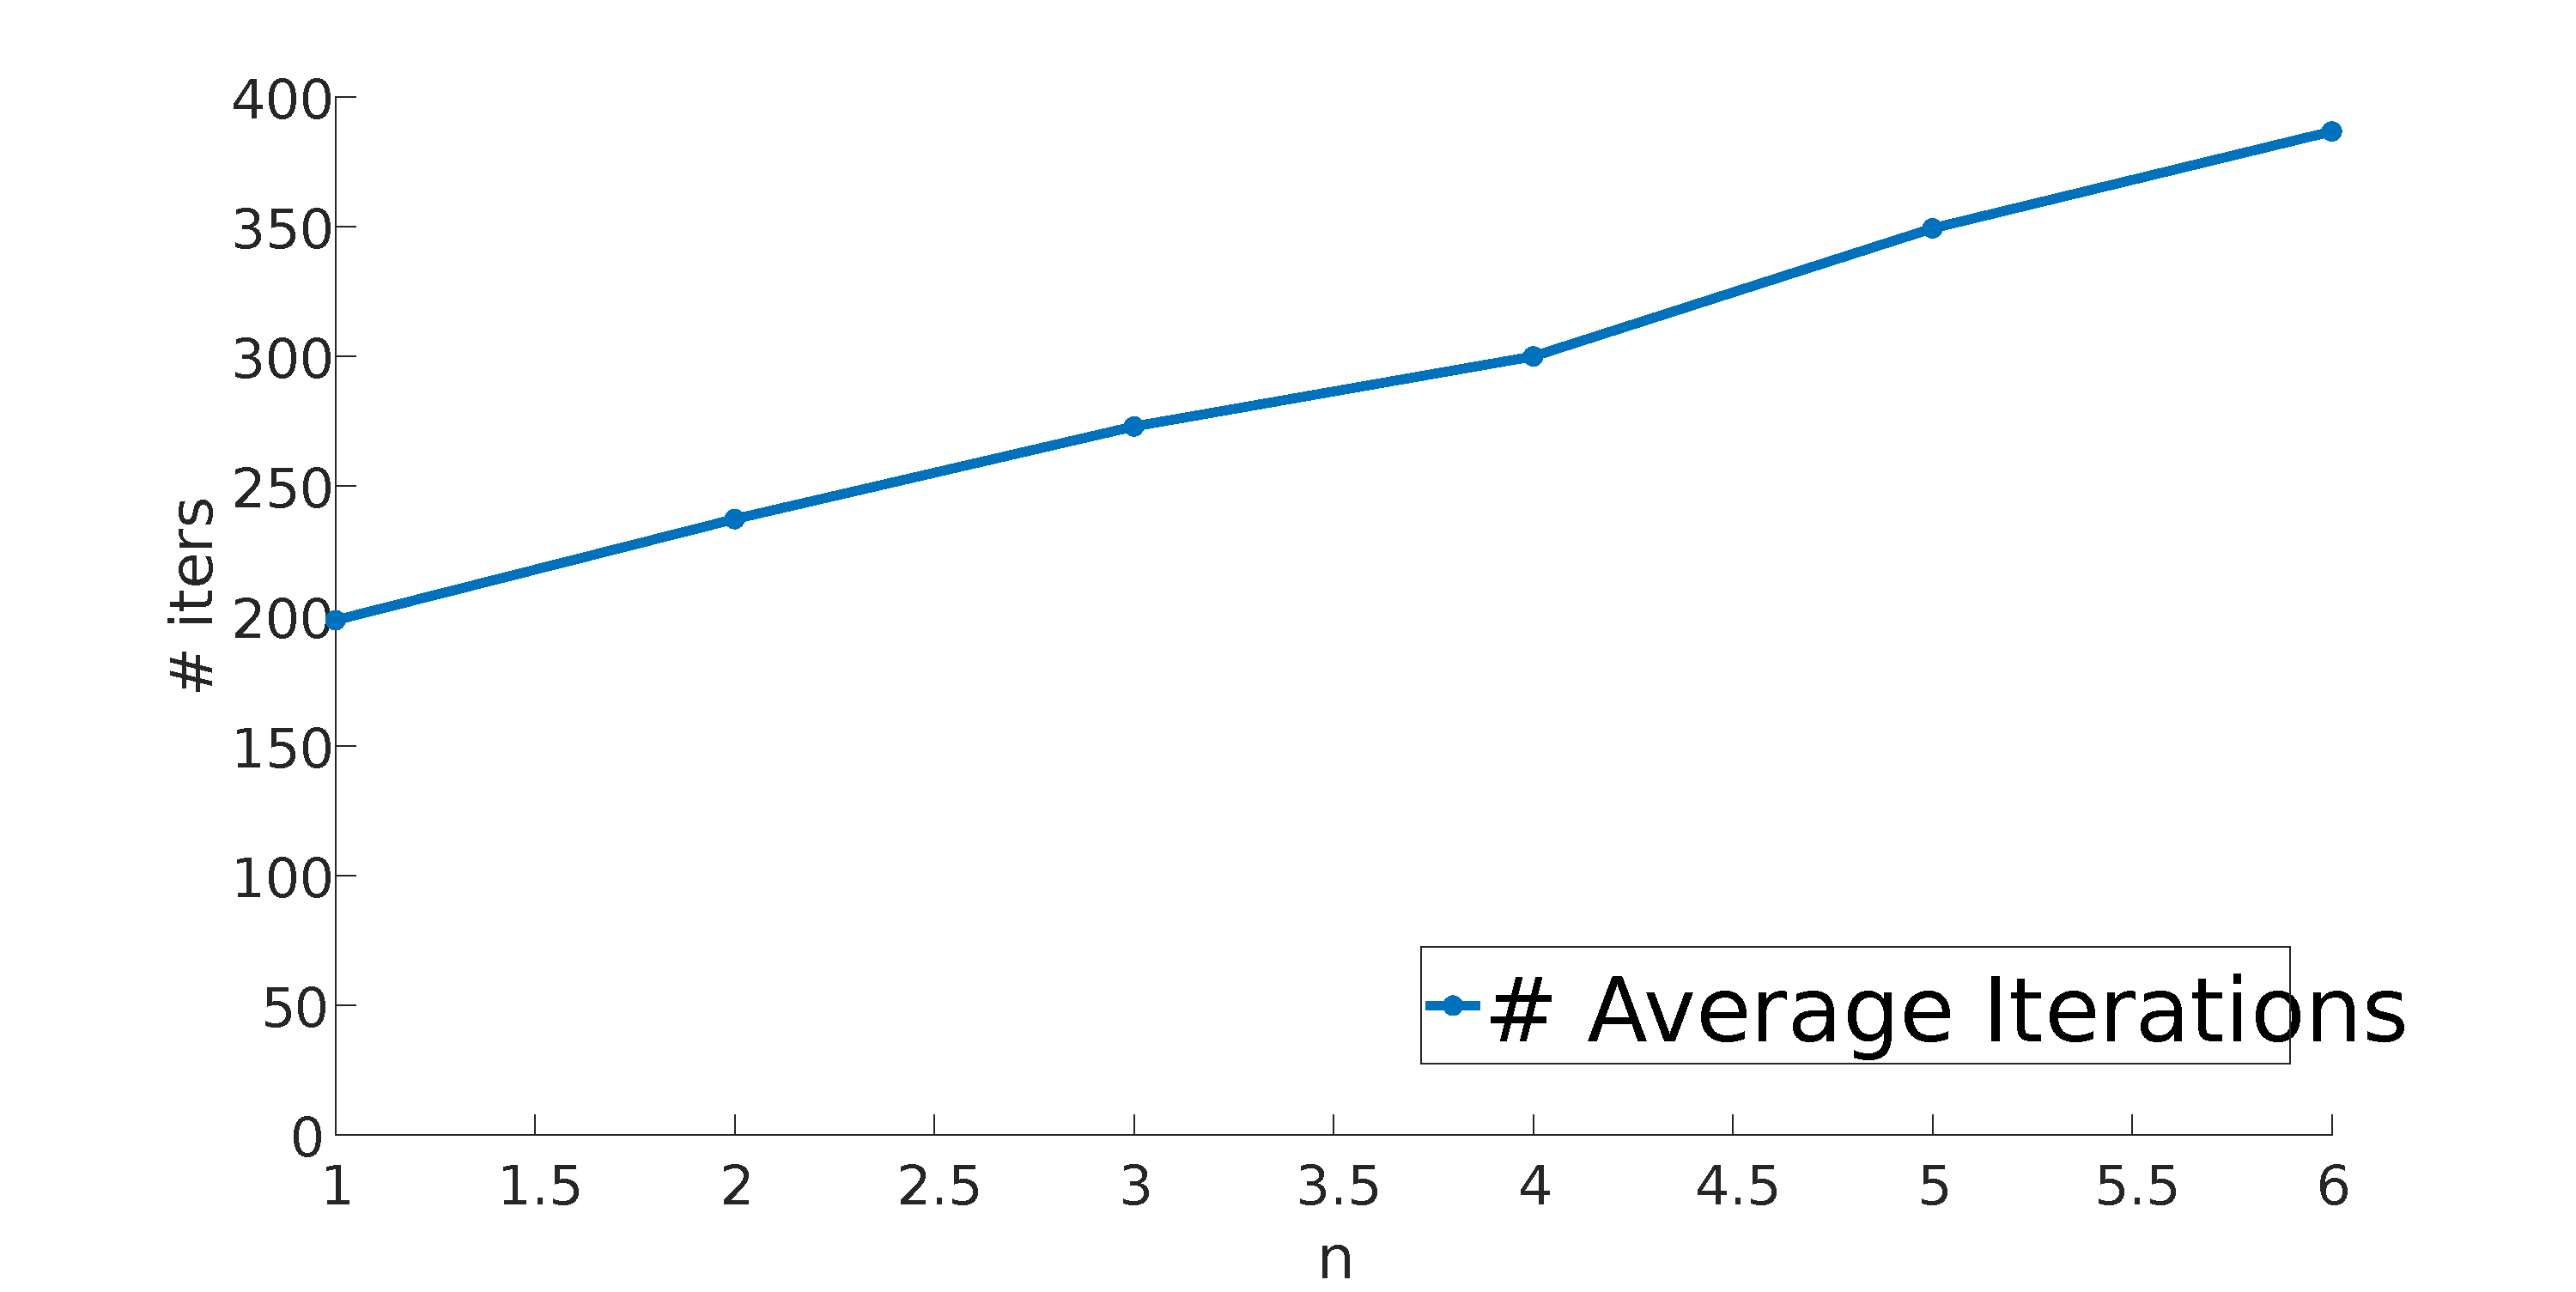
\includegraphics[width=2.5in]{images/penalty_iters.pdf}
		\caption*{(b)}
		\label{sfig:pen_iters}
	\end{subfigure}%
	\caption{\textbf{Penalty Function Performance}: A plot of penalty functions $U_n$ of different orders $n$ from 1 to 6. }
	\label{fig:penalty_comparison}
\end{figure}